\documentclass{standalone}
\usepackage{tikz}
\usetikzlibrary{patterns, positioning}


\begin{document}
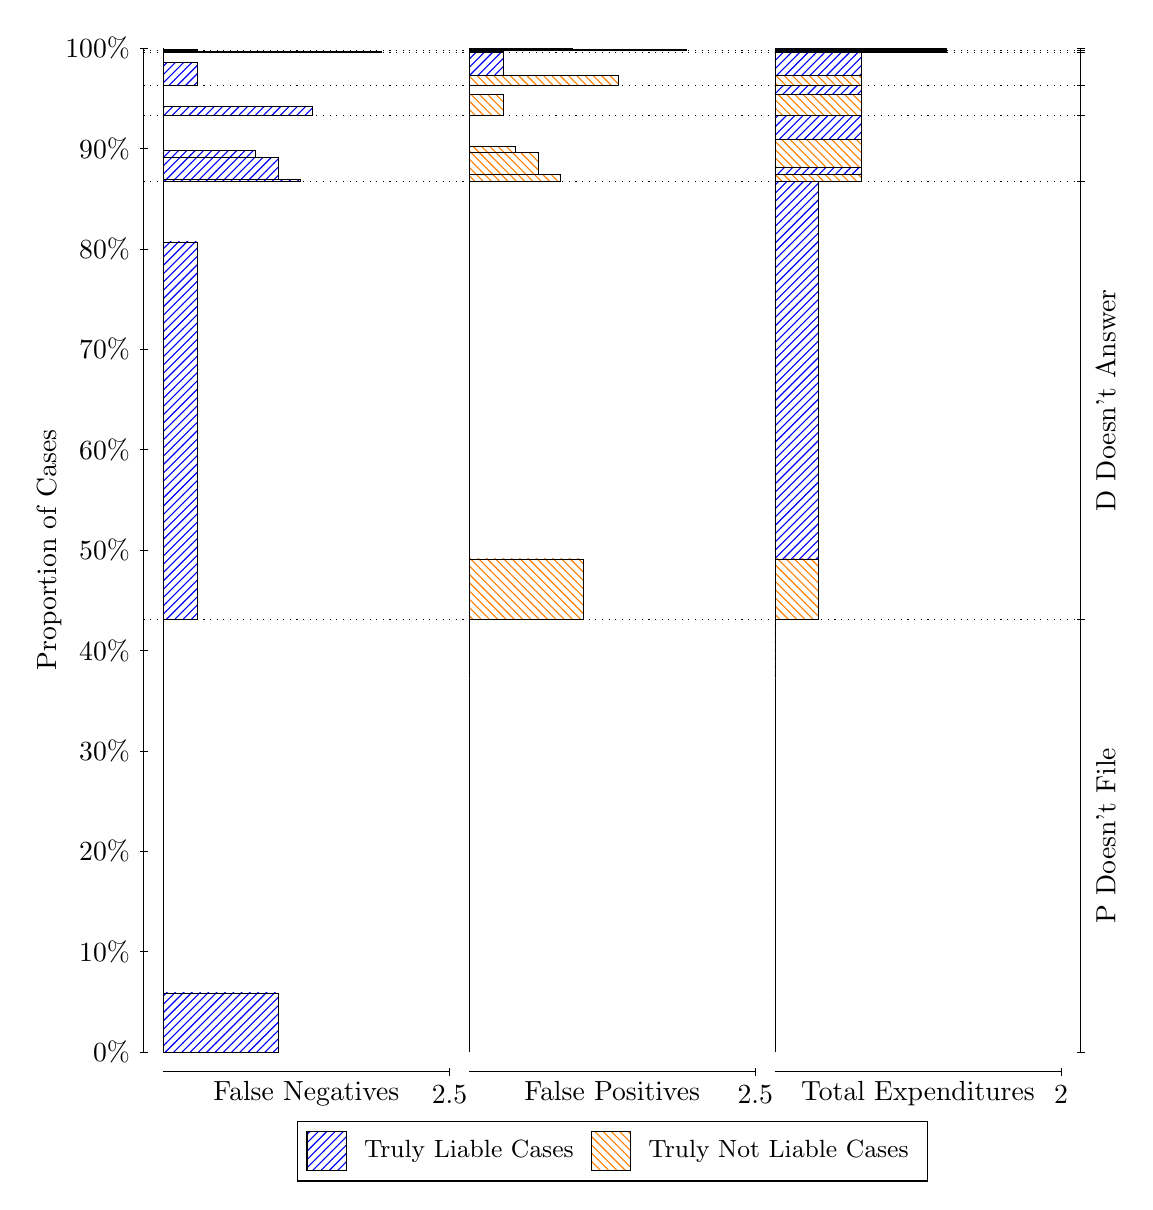
\begin{tikzpicture}
\draw[black, very thin] (1.5,1.75) -- (1.5,14.5);
\node[rotate=90, text=black, anchor=center] at (0.3, 8.125) {Proportion of Cases};
\draw[black, very thin] (1.45,1.75) -- (1.55,1.75);
\node[text=black, anchor=east] at (1.45, 1.75) {0\%};
\draw[black, very thin] (1.45,3.025) -- (1.55,3.025);
\node[text=black, anchor=east] at (1.45, 3.025) {10\%};
\draw[black, very thin] (1.45,4.3) -- (1.55,4.3);
\node[text=black, anchor=east] at (1.45, 4.3) {20\%};
\draw[black, very thin] (1.45,5.575) -- (1.55,5.575);
\node[text=black, anchor=east] at (1.45, 5.575) {30\%};
\draw[black, very thin] (1.45,6.85) -- (1.55,6.85);
\node[text=black, anchor=east] at (1.45, 6.85) {40\%};
\draw[black, very thin] (1.45,8.125) -- (1.55,8.125);
\node[text=black, anchor=east] at (1.45, 8.125) {50\%};
\draw[black, very thin] (1.45,9.4) -- (1.55,9.4);
\node[text=black, anchor=east] at (1.45, 9.4) {60\%};
\draw[black, very thin] (1.45,10.675) -- (1.55,10.675);
\node[text=black, anchor=east] at (1.45, 10.675) {70\%};
\draw[black, very thin] (1.45,11.95) -- (1.55,11.95);
\node[text=black, anchor=east] at (1.45, 11.95) {80\%};
\draw[black, very thin] (1.45,13.225) -- (1.55,13.225);
\node[text=black, anchor=east] at (1.45, 13.225) {90\%};
\draw[black, very thin] (1.45,14.5) -- (1.55,14.5);
\node[text=black, anchor=east] at (1.45, 14.5) {100\%};

\draw[black, very thin] (13.4,1.75) -- (13.4,14.5);
\draw[black, very thin] (13.35,1.75) -- (13.45,1.75);
\node[anchor=west] at (13.35, 1.75) {};
\draw[black, very thin] (13.35,7.2445) -- (13.45,7.2445);
\node[anchor=west] at (13.35, 7.2445) {};
\draw[black, very thin] (13.35,12.804) -- (13.45,12.804);
\node[anchor=west] at (13.35, 12.804) {};
\draw[black, very thin] (13.35,13.645) -- (13.45,13.645);
\node[anchor=west] at (13.35, 13.645) {};
\draw[black, very thin] (13.35,14.022) -- (13.45,14.022);
\node[anchor=west] at (13.35, 14.022) {};
\draw[black, very thin] (13.35,14.444) -- (13.45,14.444);
\node[anchor=west] at (13.35, 14.444) {};
\draw[black, very thin] (13.35,14.472) -- (13.45,14.472);
\node[anchor=west] at (13.35, 14.472) {};
\draw[black, very thin] (13.35,14.5) -- (13.45,14.5);
\node[anchor=west] at (13.35, 14.5) {};

\draw[black, very thin, pattern color=blue, pattern=north east lines] (1.75,1.75) rectangle (3.2033,2.5);
\draw[black, very thin, pattern color=orange, pattern=north west lines] (1.75,2.5) rectangle (1.75,7.2445);
\draw[black, very thin, pattern color=blue, pattern=north east lines] (1.75,7.2445) rectangle (2.186,12.037);
\draw[black, very thin, pattern color=orange, pattern=north west lines] (1.75,12.037) rectangle (1.75,12.804);
\draw[black, very thin, pattern color=blue, pattern=north east lines] (1.75,12.804) rectangle (3.494,12.835);
\draw[black, very thin, pattern color=blue, pattern=north east lines] (1.75,12.835) rectangle (3.2033,13.113);
\draw[black, very thin, pattern color=blue, pattern=north east lines] (1.75,13.113) rectangle (2.9127,13.201);
\draw[black, very thin, pattern color=orange, pattern=north west lines] (1.75,13.201) rectangle (1.75,13.645);
\draw[black, very thin, pattern color=blue, pattern=north east lines] (1.75,13.645) rectangle (3.6393,13.76);
\draw[black, very thin, pattern color=orange, pattern=north west lines] (1.75,13.76) rectangle (1.75,14.022);
\draw[black, very thin, pattern color=blue, pattern=north east lines] (1.75,14.022) rectangle (2.186,14.314);
\draw[black, very thin, pattern color=orange, pattern=north west lines] (1.75,14.314) rectangle (1.75,14.444);
\draw[black, very thin, pattern color=blue, pattern=north east lines] (1.75,14.444) rectangle (4.5113,14.457);
\draw[black, very thin, pattern color=orange, pattern=north west lines] (1.75,14.457) rectangle (1.75,14.472);
\draw[black, very thin, pattern color=blue, pattern=north east lines] (1.75,14.472) rectangle (2.186,14.487);
\draw[black, very thin, pattern color=orange, pattern=north west lines] (1.75,14.487) rectangle (1.75,14.5);
\draw[black, very thin, pattern color=orange, pattern=north west lines] (5.6333,1.75) rectangle (5.6333,6.4945);
\draw[black, very thin, pattern color=blue, pattern=north east lines] (5.6333,6.4945) rectangle (5.6333,7.2445);
\draw[black, very thin, pattern color=orange, pattern=north west lines] (5.6333,7.2445) rectangle (7.0867,8.0113);
\draw[black, very thin, pattern color=blue, pattern=north east lines] (5.6333,8.0113) rectangle (5.6333,12.804);
\draw[black, very thin, pattern color=orange, pattern=north west lines] (5.6333,12.804) rectangle (6.796,12.892);
\draw[black, very thin, pattern color=orange, pattern=north west lines] (5.6333,12.892) rectangle (6.5053,13.176);
\draw[black, very thin, pattern color=orange, pattern=north west lines] (5.6333,13.176) rectangle (6.2147,13.247);
\draw[black, very thin, pattern color=blue, pattern=north east lines] (5.6333,13.247) rectangle (5.6333,13.645);
\draw[black, very thin, pattern color=orange, pattern=north west lines] (5.6333,13.645) rectangle (6.0693,13.907);
\draw[black, very thin, pattern color=blue, pattern=north east lines] (5.6333,13.907) rectangle (5.6333,14.022);
\draw[black, very thin, pattern color=orange, pattern=north west lines] (5.6333,14.022) rectangle (7.5227,14.152);
\draw[black, very thin, pattern color=blue, pattern=north east lines] (5.6333,14.152) rectangle (6.0693,14.444);
\draw[black, very thin, pattern color=orange, pattern=north west lines] (5.6333,14.444) rectangle (6.0693,14.458);
\draw[black, very thin, pattern color=blue, pattern=north east lines] (5.6333,14.458) rectangle (5.6333,14.472);
\draw[black, very thin, pattern color=orange, pattern=north west lines] (5.6333,14.472) rectangle (8.3947,14.485);
\draw[black, very thin, pattern color=blue, pattern=north east lines] (5.6333,14.485) rectangle (6.9413,14.5);
\draw[black, very thin, pattern color=orange, pattern=north west lines] (9.5167,1.75) rectangle (9.5167,6.4945);
\draw[black, very thin, pattern color=blue, pattern=north east lines] (9.5167,6.4945) rectangle (9.5167,7.2445);
\draw[black, very thin, pattern color=orange, pattern=north west lines] (9.5167,7.2445) rectangle (10.062,8.0113);
\draw[black, very thin, pattern color=blue, pattern=north east lines] (9.5167,8.0113) rectangle (10.062,12.804);
\draw[black, very thin, pattern color=orange, pattern=north west lines] (9.5167,12.804) rectangle (10.607,12.892);
\draw[black, very thin, pattern color=blue, pattern=north east lines] (9.5167,12.892) rectangle (10.607,12.98);
\draw[black, very thin, pattern color=orange, pattern=north west lines] (9.5167,12.98) rectangle (10.607,13.336);
\draw[black, very thin, pattern color=blue, pattern=north east lines] (9.5167,13.336) rectangle (10.607,13.645);
\draw[black, very thin, pattern color=orange, pattern=north west lines] (9.5167,13.645) rectangle (10.607,13.907);
\draw[black, very thin, pattern color=blue, pattern=north east lines] (9.5167,13.907) rectangle (10.607,14.022);
\draw[black, very thin, pattern color=orange, pattern=north west lines] (9.5167,14.022) rectangle (10.607,14.152);
\draw[black, very thin, pattern color=blue, pattern=north east lines] (9.5167,14.152) rectangle (10.607,14.444);
\draw[black, very thin, pattern color=orange, pattern=north west lines] (9.5167,14.444) rectangle (11.697,14.458);
\draw[black, very thin, pattern color=blue, pattern=north east lines] (9.5167,14.458) rectangle (11.697,14.472);
\draw[black, very thin, pattern color=orange, pattern=north west lines] (9.5167,14.472) rectangle (11.697,14.485);
\draw[black, very thin, pattern color=blue, pattern=north east lines] (9.5167,14.485) rectangle (11.697,14.5);
\draw[black, dotted] (1.5,7.2445) -- (13.4,7.2445);
\draw[black, dotted] (1.5,12.804) -- (13.4,12.804);
\draw[black, dotted] (1.5,13.645) -- (13.4,13.645);
\draw[black, dotted] (1.5,14.022) -- (13.4,14.022);
\draw[black, dotted] (1.5,14.444) -- (13.4,14.444);
\draw[black, dotted] (1.5,14.472) -- (13.4,14.472);
\draw[black, very thin] (1.75,1.5) -- (5.3833,1.5);
\node[text=black, anchor=north] at (3.5667, 1.5) {False Negatives};
\draw[black, very thin] (5.3833,1.45) -- (5.3833,1.55);
\node[text=black, anchor=north] at (5.3833, 1.45) {2.5};

\draw[black, very thin] (5.6333,1.5) -- (9.2667,1.5);
\node[text=black, anchor=north] at (7.45, 1.5) {False Positives};
\draw[black, very thin] (9.2667,1.45) -- (9.2667,1.55);
\node[text=black, anchor=north] at (9.2667, 1.45) {2.5};

\draw[black, very thin] (9.5167,1.5) -- (13.15,1.5);
\node[text=black, anchor=north] at (11.333, 1.5) {Total Expenditures};
\draw[black, very thin] (13.15,1.45) -- (13.15,1.55);
\node[text=black, anchor=north] at (13.15, 1.45) {2};

\node[text=black, centered, rotate=90] at (13.72, 4.4972) {P Doesn't File};
\node[text=black, centered, rotate=90] at (13.72, 10.024) {D Doesn't Answer};






\draw (7.449999999999999,1.5) node[draw=none] (baseCoordinate) {};
\begin{scope}[align=center]
        \matrix[scale=0.5, draw=black, below=0.5cm of baseCoordinate, nodes={draw}, column sep=0.1cm]{
            \node[rectangle, draw, minimum width=0.5cm, minimum height=0.5cm, pattern color=blue, pattern=north east lines] {}; &
            \node[draw=none, font=\small, text=black] (B) {Truly Liable Cases}; &
            \node[rectangle, draw, minimum width=0.5cm, minimum height=0.5cm, pattern color=orange, pattern=north west lines] {}; &
            \node[draw=none, font=\small, text=black] (B) {Truly Not Liable Cases}; \\
            };
\end{scope}

\end{tikzpicture}
\end{document}